\documentclass[tikz,border=20pt]{standalone}
\usepackage{tikz}
\usepackage{amsmath}
\usepackage{amssymb}
\usetikzlibrary{shapes.geometric, arrows.meta, positioning, calc, backgrounds, fit, shadows.blur}

% Color Definitions
\definecolor{navyDark}{HTML}{0B2545}
\definecolor{navyLight}{HTML}{EEF4F8}
\definecolor{navyBorder}{HTML}{134074}

\definecolor{emeraldDark}{HTML}{0E6251}
\definecolor{emeraldLight}{HTML}{E8F8F5}
\definecolor{emeraldBorder}{HTML}{16A085}

\definecolor{purpleDark}{HTML}{512E5F}
\definecolor{purpleLight}{HTML}{F5EEF8}
\definecolor{purpleBorder}{HTML}{8E44AD}

\definecolor{amberDark}{HTML}{7D6608}
\definecolor{amberLight}{HTML}{FEF9E7}
\definecolor{amberBorder}{HTML}{D4AC0D}

\definecolor{crimsonDark}{HTML}{78281F}
\definecolor{crimsonLight}{HTML}{FDEDEC}
\definecolor{crimsonBorder}{HTML}{C0392B}

\definecolor{slateDark}{HTML}{2C3E50}
\definecolor{slateLight}{HTML}{F8F9FA}
\definecolor{slateBorder}{HTML}{BDC3C7}

\begin{document}
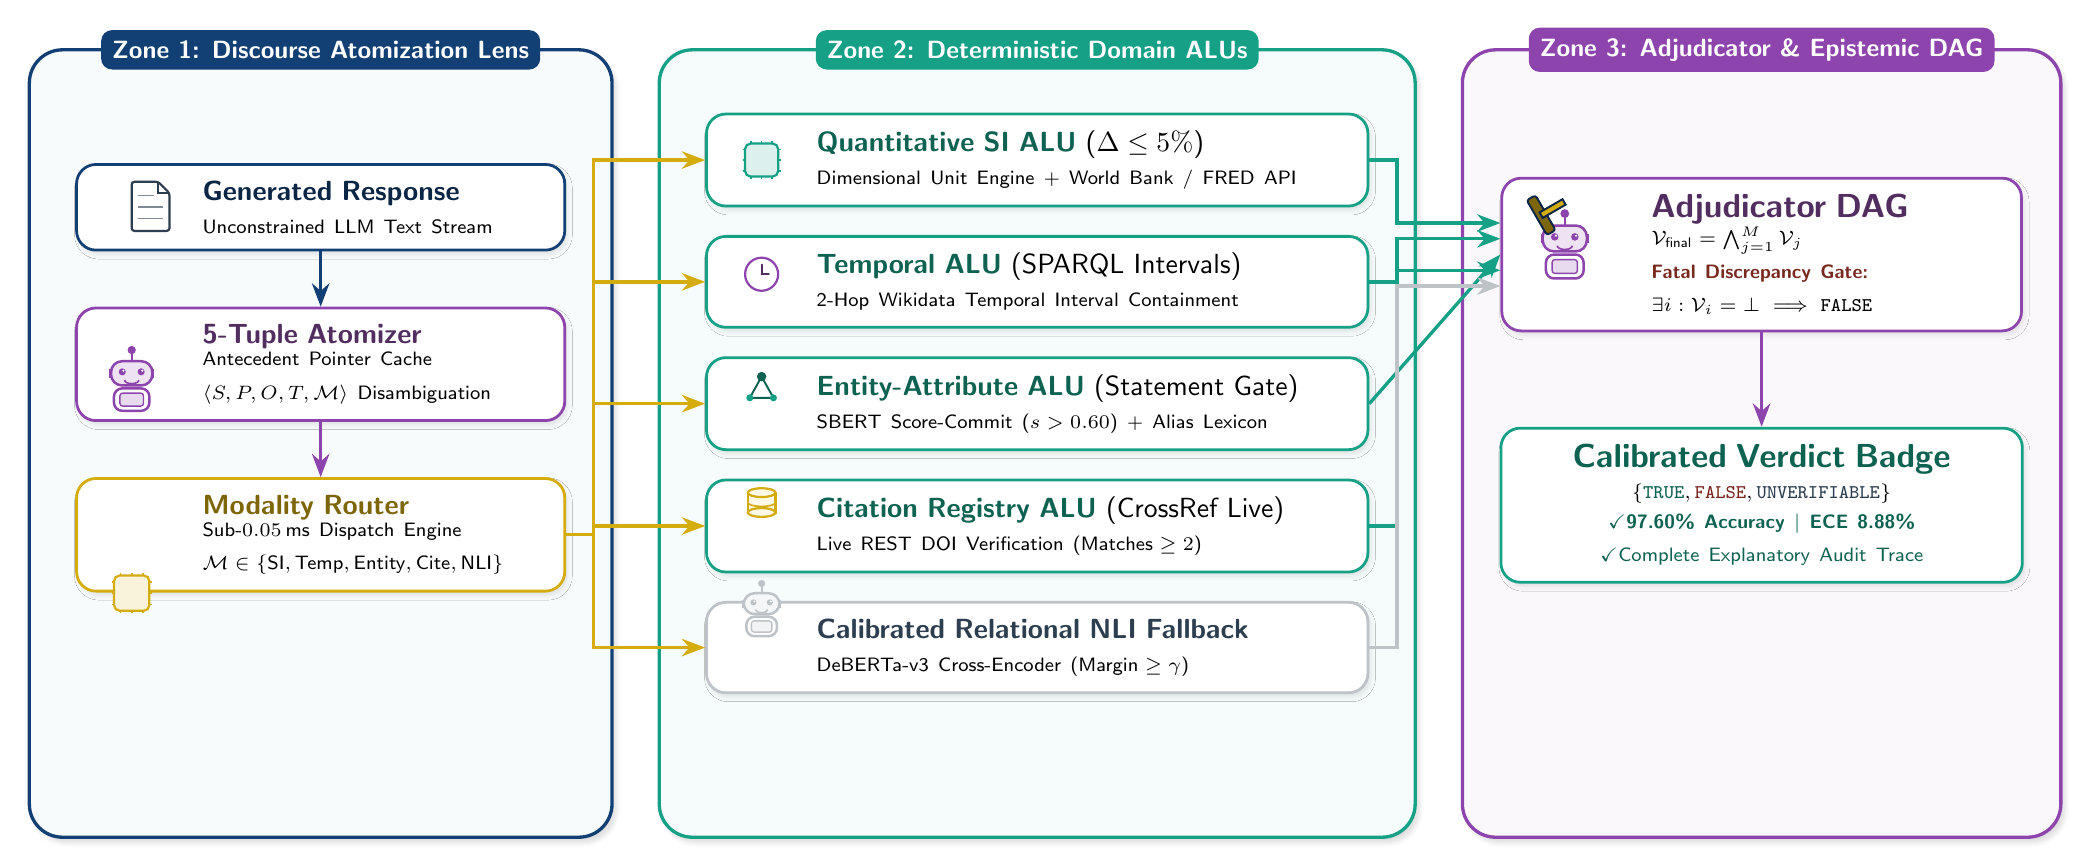
\begin{tikzpicture}[
    font=\sffamily,
    >=Stealth,
    zonebox/.style={
        draw=#1Border, fill=#1Light!40, line width=1.2pt, rounded corners=12pt,
        blur shadow={shadow blur steps=6, shadow xshift=1.5pt, shadow yshift=-2pt, shadow opacity=14}
    },
    card/.style={
        draw=#1Border, fill=white, line width=1.0pt, rounded corners=7pt,
        blur shadow={shadow blur steps=4, shadow xshift=1pt, shadow yshift=-1.5pt, shadow opacity=10},
        align=left, inner sep=6pt
    },
    wire/.style={
        ->, line width=1.2pt, draw=#1Border
    }
]

% ==================== VECTOR ICONS ====================
\newcommand{\drawDocIcon}[3]{%
    \begin{scope}[shift={(#1,#2)}, scale=#3]
        \draw[fill=white, draw=slateDark, line width=0.8pt, rounded corners=1pt] 
            (0,0) -- (0.6,0) -- (0.6,0.6) -- (0.42,0.78) -- (0,0.78) -- cycle;
        \draw[draw=slateDark, line width=0.6pt] (0.42,0.78) -- (0.42,0.6) -- (0.6,0.6);
        \draw[draw=slateDark!60, line width=0.5pt] (0.1,0.56) -- (0.35,0.56);
        \draw[draw=slateDark!60, line width=0.5pt] (0.1,0.38) -- (0.5,0.38);
        \draw[draw=slateDark!60, line width=0.5pt] (0.1,0.2) -- (0.5,0.2);
    \end{scope}
}

\newcommand{\drawRobotAgent}[4]{%
    \begin{scope}[shift={(#1,#2)}, scale=#3]
        \draw[line width=0.8pt, draw=#4] (0, 0.42) -- (0, 0.62);
        \fill[#4] (0, 0.65) circle (0.07);
        \draw[fill=#4!15, draw=#4, line width=0.9pt, rounded corners=4pt] (-0.35, 0.05) rectangle (0.35, 0.46);
        \fill[#4] (-0.38, 0.18) rectangle (-0.33, 0.33);
        \fill[#4] (0.33, 0.18) rectangle (0.38, 0.33);
        \fill[#4] (-0.16, 0.28) circle (0.06);
        \fill[#4] (0.16, 0.28) circle (0.06);
        \fill[white] (-0.14, 0.3) circle (0.02);
        \fill[white] (0.18, 0.3) circle (0.02);
        \draw[draw=#4, line width=0.6pt] (-0.12, 0.14) arc (180:360:0.12 and 0.06);
        \draw[fill=white, draw=#4, line width=0.9pt, rounded corners=3pt] (-0.3, -0.38) rectangle (0.3, 0.0);
        \draw[fill=#4!20, draw=#4, line width=0.5pt, rounded corners=1pt] (-0.2, -0.3) rectangle (0.2, -0.08);
    \end{scope}
}

\newcommand{\drawDatabaseIcon}[3]{%
    \begin{scope}[shift={(#1,#2)}, scale=#3]
        \draw[fill=amberLight, draw=amberBorder, line width=0.8pt] (-0.25, -0.18) rectangle (0.25, 0.18);
        \draw[fill=amberLight, draw=amberBorder, line width=0.8pt] (0, 0.18) ellipse (0.25 and 0.08);
        \draw[fill=amberLight, draw=amberBorder, line width=0.8pt] (0, -0.18) ellipse (0.25 and 0.08);
        \draw[draw=amberBorder, line width=0.6pt] (-0.25, 0.0) arc (180:360:0.25 and 0.07);
    \end{scope}
}

\newcommand{\drawGavelIcon}[3]{%
    \begin{scope}[shift={(#1,#2)}, scale=#3, rotate=30]
        \draw[fill=amberDark, draw=navyDark, line width=0.7pt, rounded corners=1pt] (-0.08, -0.32) rectangle (0.08, 0.32);
        \draw[fill=amberBorder, draw=navyDark, line width=0.7pt] (0, -0.05) rectangle (0.42, 0.05);
    \end{scope}
}

\newcommand{\drawChipIcon}[4]{%
    \begin{scope}[shift={(#1,#2)}, scale=#3]
        \draw[fill=#4!15, draw=#4, line width=0.8pt, rounded corners=2pt] (-0.28, -0.28) rectangle (0.28, 0.28);
        \draw[draw=#4, line width=0.6pt] (-0.18, 0.32) -- (-0.18, 0.28) (0.0, 0.32) -- (0.0, 0.28) (0.18, 0.32) -- (0.18, 0.28);
        \draw[draw=#4, line width=0.6pt] (-0.18, -0.32) -- (-0.18, -0.28) (0.0, -0.32) -- (0.0, -0.28) (0.18, -0.32) -- (0.18, -0.28);
        \draw[draw=#4, line width=0.6pt] (-0.32, -0.18) -- (-0.28, -0.18) (-0.32, 0.0) -- (-0.28, 0.0) (-0.32, 0.18) -- (-0.28, 0.18);
        \draw[draw=#4, line width=0.6pt] (0.32, -0.18) -- (0.28, -0.18) (0.32, 0.0) -- (0.28, 0.0) (0.32, 0.18) -- (0.28, 0.18);
    \end{scope}
}

\newcommand{\drawClockIcon}[3]{%
    \begin{scope}[shift={(#1,#2)}, scale=#3]
        \draw[fill=white, draw=purpleBorder, line width=0.8pt] (0,0) circle (0.28);
        \draw[draw=purpleDark, line width=0.8pt, line cap=round] (0,0) -- (0, 0.16);
        \draw[draw=purpleDark, line width=0.8pt, line cap=round] (0,0) -- (0.12, 0);
    \end{scope}
}

\newcommand{\drawGraphIcon}[3]{%
    \begin{scope}[shift={(#1,#2)}, scale=#3]
        \draw[draw=emeraldDark, line width=0.7pt] (-0.2,-0.16) -- (0.2,-0.16) -- (0, 0.2) -- cycle;
        \fill[emeraldBorder] (-0.2,-0.16) circle (0.06);
        \fill[emeraldBorder] (0.2,-0.16) circle (0.06);
        \fill[emeraldDark] (0, 0.2) circle (0.08);
    \end{scope}
}


% ==================== ZONE 1 ====================
\draw[zonebox=navy] (-0.4, -5.6) rectangle (7.0, 4.4);
\node[fill=navyBorder, text=white, font=\bfseries\sffamily\small, rounded corners=4pt, inner sep=4pt] at (3.3, 4.4) {Zone 1: Discourse Atomization Lens};

\node[card=navy, minimum width=6.2cm, text width=4.8cm] (z1_doc) at (3.3, 2.4) {
    \hspace*{0.9cm}\textbf{\color{navyDark} Generated Response}\\
    \hspace*{0.9cm}\scriptsize Unconstrained LLM Text Stream
};
\drawDocIcon{0.9}{2.1}{0.8}

\node[card=purple, below=0.7cm of z1_doc, minimum width=6.2cm, text width=4.8cm] (z1_atom) {
    \hspace*{0.9cm}\textbf{\color{purpleDark} 5-Tuple Atomizer}\\
    \hspace*{0.9cm}\scriptsize Antecedent Pointer Cache\\
    \hspace*{0.9cm}\scriptsize $\langle S, P, O, T, \mathcal{M} \rangle$ Disambiguation
};
\drawRobotAgent{0.9}{0.1}{0.75}{purpleBorder}

\node[card=amber, below=0.7cm of z1_atom, minimum width=6.2cm, text width=4.8cm] (z1_router) {
    \hspace*{0.9cm}\textbf{\color{amberDark} Modality Router}\\
    \hspace*{0.9cm}\scriptsize Sub-$0.05\,\text{ms}$ Dispatch Engine\\
    \hspace*{0.9cm}\scriptsize $\mathcal{M} \in \{\text{SI}, \text{Temp}, \text{Entity}, \text{Cite}, \text{NLI}\}$
};
\drawChipIcon{0.9}{-2.5}{0.8}{amberBorder}

\draw[wire=navy] (z1_doc) -- (z1_atom);
\draw[wire=purple] (z1_atom) -- (z1_router);


% ==================== ZONE 2 ====================
\draw[zonebox=emerald] (7.6, -5.6) rectangle (17.2, 4.4);
\node[fill=emeraldBorder, text=white, font=\bfseries\sffamily\small, rounded corners=4pt, inner sep=4pt] at (12.4, 4.4) {Zone 2: Deterministic Domain ALUs};

\node[card=emerald, minimum width=8.4cm, text width=7.2cm] (alu1) at (12.4, 3.0) {
    \hspace*{0.8cm}\textbf{\color{emeraldDark} Quantitative SI ALU} ($\Delta \le 5\%$)\\
    \hspace*{0.8cm}\scriptsize Dimensional Unit Engine + World Bank / FRED API
};
\drawChipIcon{8.9}{3.0}{0.75}{emeraldBorder}

\node[card=emerald, below=0.35cm of alu1, minimum width=8.4cm, text width=7.2cm] (alu2) {
    \hspace*{0.8cm}\textbf{\color{emeraldDark} Temporal ALU} (SPARQL Intervals)\\
    \hspace*{0.8cm}\scriptsize 2-Hop Wikidata Temporal Interval Containment
};
\drawClockIcon{8.9}{1.55}{0.75}

\node[card=emerald, below=0.35cm of alu2, minimum width=8.4cm, text width=7.2cm] (alu3) {
    \hspace*{0.8cm}\textbf{\color{emeraldDark} Entity-Attribute ALU} (Statement Gate)\\
    \hspace*{0.8cm}\scriptsize SBERT Score-Commit ($s > 0.60$) + Alias Lexicon
};
\drawGraphIcon{8.9}{0.1}{0.75}

\node[card=emerald, below=0.35cm of alu3, minimum width=8.4cm, text width=7.2cm] (alu4) {
    \hspace*{0.8cm}\textbf{\color{emeraldDark} Citation Registry ALU} (CrossRef Live)\\
    \hspace*{0.8cm}\scriptsize Live REST DOI Verification ($\text{Matches} \ge 2$)
};
\drawDatabaseIcon{8.9}{-1.35}{0.7}

\node[card=slate, below=0.35cm of alu4, minimum width=8.4cm, text width=7.2cm] (alu5) {
    \hspace*{0.8cm}\textbf{\color{slateDark} Calibrated Relational NLI Fallback}\\
    \hspace*{0.8cm}\scriptsize DeBERTa-v3 Cross-Encoder ($\text{Margin} \ge \gamma$)
};
\drawRobotAgent{8.9}{-2.8}{0.65}{slateBorder}

% Connectors from Router to ALUs
\draw[wire=amber] (z1_router.east) -- ++(0.35,0) |- (alu1.west);
\draw[wire=amber] (z1_router.east) -- ++(0.35,0) |- (alu2.west);
\draw[wire=amber] (z1_router.east) -- ++(0.35,0) |- (alu3.west);
\draw[wire=amber] (z1_router.east) -- ++(0.35,0) |- (alu4.west);
\draw[wire=amber] (z1_router.east) -- ++(0.35,0) |- (alu5.west);


% ==================== ZONE 3 ====================
\draw[zonebox=purple] (17.8, -5.6) rectangle (25.4, 4.4);
\node[fill=purpleBorder, text=white, font=\bfseries\sffamily\small, rounded corners=4pt, inner sep=4pt] at (21.6, 4.4) {Zone 3: Adjudicator \& Epistemic DAG};

% Adjudicator Card with Integrated Avatar & Gavel
\node[card=purple, minimum width=6.6cm, text width=5.0cm] (dag_card) at (21.6, 1.8) {
    \hspace*{1.1cm}\textbf{\color{purpleDark}\large Adjudicator DAG}\\
    \hspace*{1.1cm}\scriptsize $\mathcal{V}_{\text{final}} = \bigwedge_{j=1}^M \mathcal{V}_j$\\[3pt]
    \hspace*{1.1cm}\textbf{\color{crimsonDark}\scriptsize Fatal Discrepancy Gate:}\\
    \hspace*{1.1cm}\scriptsize $\exists i: \mathcal{V}_i = \bot \implies \texttt{FALSE}$
};
\drawRobotAgent{19.1}{1.8}{0.8}{purpleBorder}
\drawGavelIcon{18.8}{2.3}{0.8}

% Parallel fan-in
\draw[wire=emerald] (alu1.east) -- ++(0.35,0) |- ($(dag_card.west) + (0, 0.4)$);
\draw[wire=emerald] (alu2.east) -- ++(0.35,0) |- ($(dag_card.west) + (0, 0.2)$);
\draw[wire=emerald] (alu3.east) -- (dag_card.west);
\draw[wire=emerald] (alu4.east) -- ++(0.35,0) |- ($(dag_card.west) - (0, 0.2)$);
\draw[wire=slate] (alu5.east) -- ++(0.35,0) |- ($(dag_card.west) - (0, 0.4)$);

% Epistemic Decision Badge
\node[card=emerald, below=1.2cm of dag_card, minimum width=6.6cm, text width=6.2cm, align=center] (verdict) {
    \textbf{\color{emeraldDark}\large Calibrated Verdict Badge}\\
    \vspace{3pt}
    \scriptsize $\{\textbf{\color{emeraldDark}\texttt{TRUE}}, \textbf{\color{crimsonDark}\texttt{FALSE}}, \textbf{\color{slateDark}\texttt{UNVERIFIABLE}}\}$\\
    \vspace{3pt}
    \textbf{\color{emeraldDark}\scriptsize \checkmark 97.60\% Accuracy $|$ ECE 8.88\%}\\
    \scriptsize \textcolor{emeraldDark}{\checkmark Complete Explanatory Audit Trace}
};

\draw[wire=purple] (dag_card.south) -- (verdict.north);

\end{tikzpicture}
\end{document}
